\documentclass[11pt]{article}
\usepackage[textwidth=18.0cm, textheight=23.0cm, top=2.0cm]{geometry}
\usepackage{pst-all}
\usepackage{amssymb}
\usepackage{tikz}
\usepackage{underscore}\begin{document}
\pagestyle{empty}


ClassName: \underline{\textbf{Class_03.2bp-27}}
\par
BinSize: \underline{\textbf{40 × 40}}
\par
ReduceSize: \underline{\textbf{40 × 40}}
\par
TypeNum: \underline{\textbf{58}}
\par
Num: \underline{\textbf{60}}
\par
OutS: \underline{\textbf{24000}}
\par
InS: \underline{\textbf{20453}}
\par
Rate: \underline{\textbf{0.852}}
\par
UB: \underline{\textbf{15}}
\par
LB0: \underline{\textbf{15}}
\par
LB: \underline{\textbf{15}}
\par
LBWithCut: \underline{\textbf{15}}
\par
NodeCut: \underline{\textbf{0}}
\par
ExtendedNodeCnt: \underline{\textbf{1}}
\par
GenNodeCnt: \underline{\textbf{1}}
\par
PrimalNode: \underline{\textbf{0}}
\par
ColumnCount: \underline{\textbf{15}}
\par
TotalCutCount: \underline{\textbf{0}}
\par
RootCutCount: \underline{\textbf{0}}
\par
LPSolverCnt: \underline{\textbf{1}}
\par
PricingSolverCnt: \underline{\textbf{0}}
\par
BranchAndBoundNum: \underline{\textbf{1}}
\par
isOpt: \underline{\textbf{true}}
\par
TimeOnInitSolution: \underline{\textbf{0.060 s}}
\par
TimeOnPrimal: \underline{\textbf{0.000 s}}
\par
TimeOnPricing: \underline{\textbf{0.000 s}}
\par
TimeOnRmp: \underline{\textbf{0.079 s}}
\par
TotalTime: \underline{\textbf{0.189 s}}
\par
\newpage


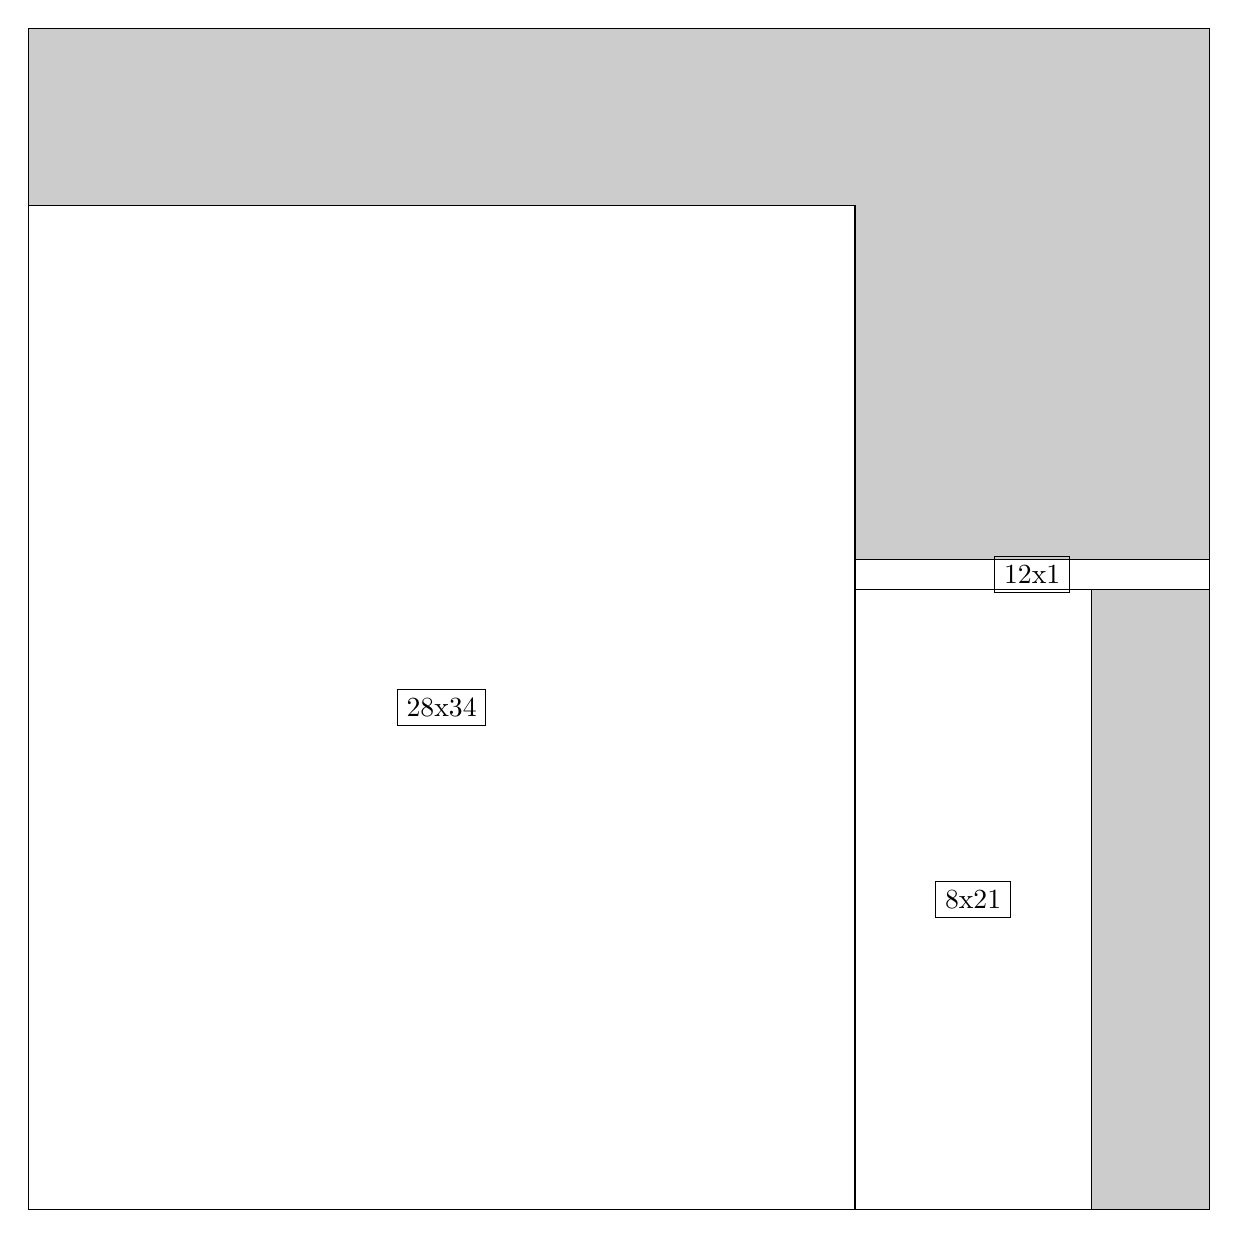
\begin{tikzpicture}[shorten >=1pt,scale=1.0,every node/.style={scale=1.0},->]
\tikzstyle{vertex}=[circle,fill=black!25,minimum size=14pt,inner sep=0pt]
\filldraw[fill=gray!40!white, draw=black] (0,0) rectangle (15.0,15.0);
\foreach \name/\x/\y/\w/\h in {28x34/0.0/0.0/10.5/12.75,8x21/10.5/0.0/3.0/7.875,12x1/10.5/7.875/4.5/0.375}
\filldraw[fill=white!40!white, draw=black] (\x,\y) rectangle node[draw] (\name) {\name} ++(\w,\h);
\end{tikzpicture}


w =28 , h =34 , x =0 , y =0 , v =952
\par
w =8 , h =21 , x =28 , y =0 , v =168
\par
w =12 , h =1 , x =28 , y =21 , v =12
\par
\newpage


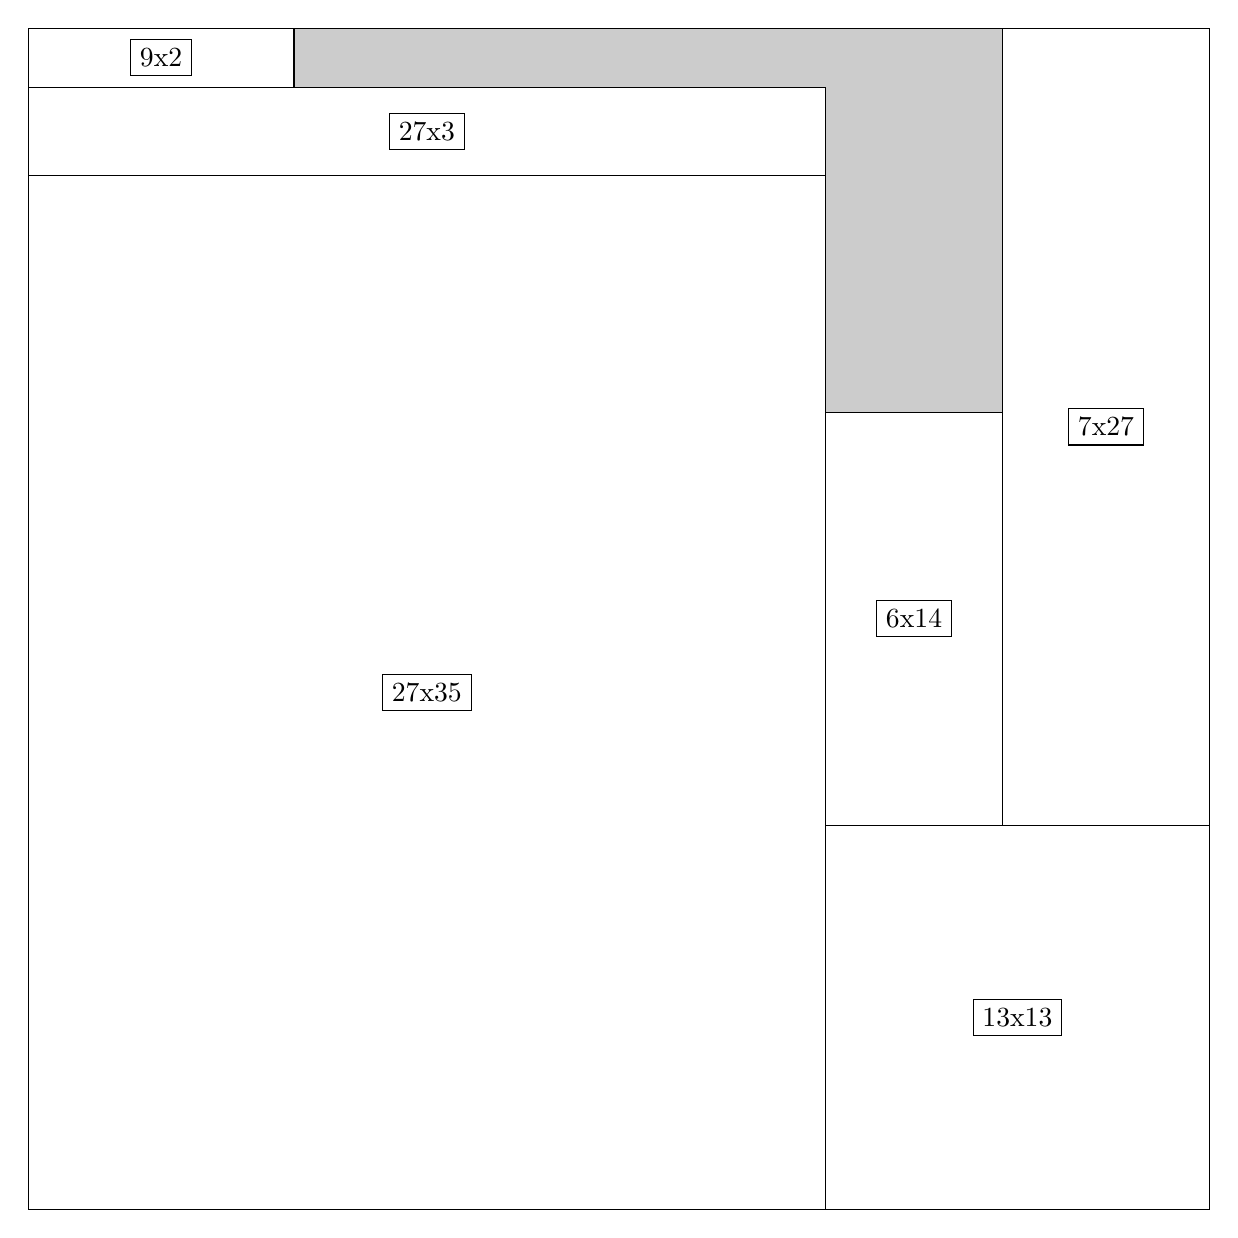
\begin{tikzpicture}[shorten >=1pt,scale=1.0,every node/.style={scale=1.0},->]
\tikzstyle{vertex}=[circle,fill=black!25,minimum size=14pt,inner sep=0pt]
\filldraw[fill=gray!40!white, draw=black] (0,0) rectangle (15.0,15.0);
\foreach \name/\x/\y/\w/\h in {27x35/0.0/0.0/10.125/13.125,7x27/12.375/4.875/2.625/10.125,13x13/10.125/0.0/4.875/4.875,6x14/10.125/4.875/2.25/5.25,27x3/0.0/13.125/10.125/1.125,9x2/0.0/14.25/3.375/0.75}
\filldraw[fill=white!40!white, draw=black] (\x,\y) rectangle node[draw] (\name) {\name} ++(\w,\h);
\end{tikzpicture}


w =27 , h =35 , x =0 , y =0 , v =945
\par
w =7 , h =27 , x =33 , y =13 , v =189
\par
w =13 , h =13 , x =27 , y =0 , v =169
\par
w =6 , h =14 , x =27 , y =13 , v =84
\par
w =27 , h =3 , x =0 , y =35 , v =81
\par
w =9 , h =2 , x =0 , y =38 , v =18
\par
\newpage


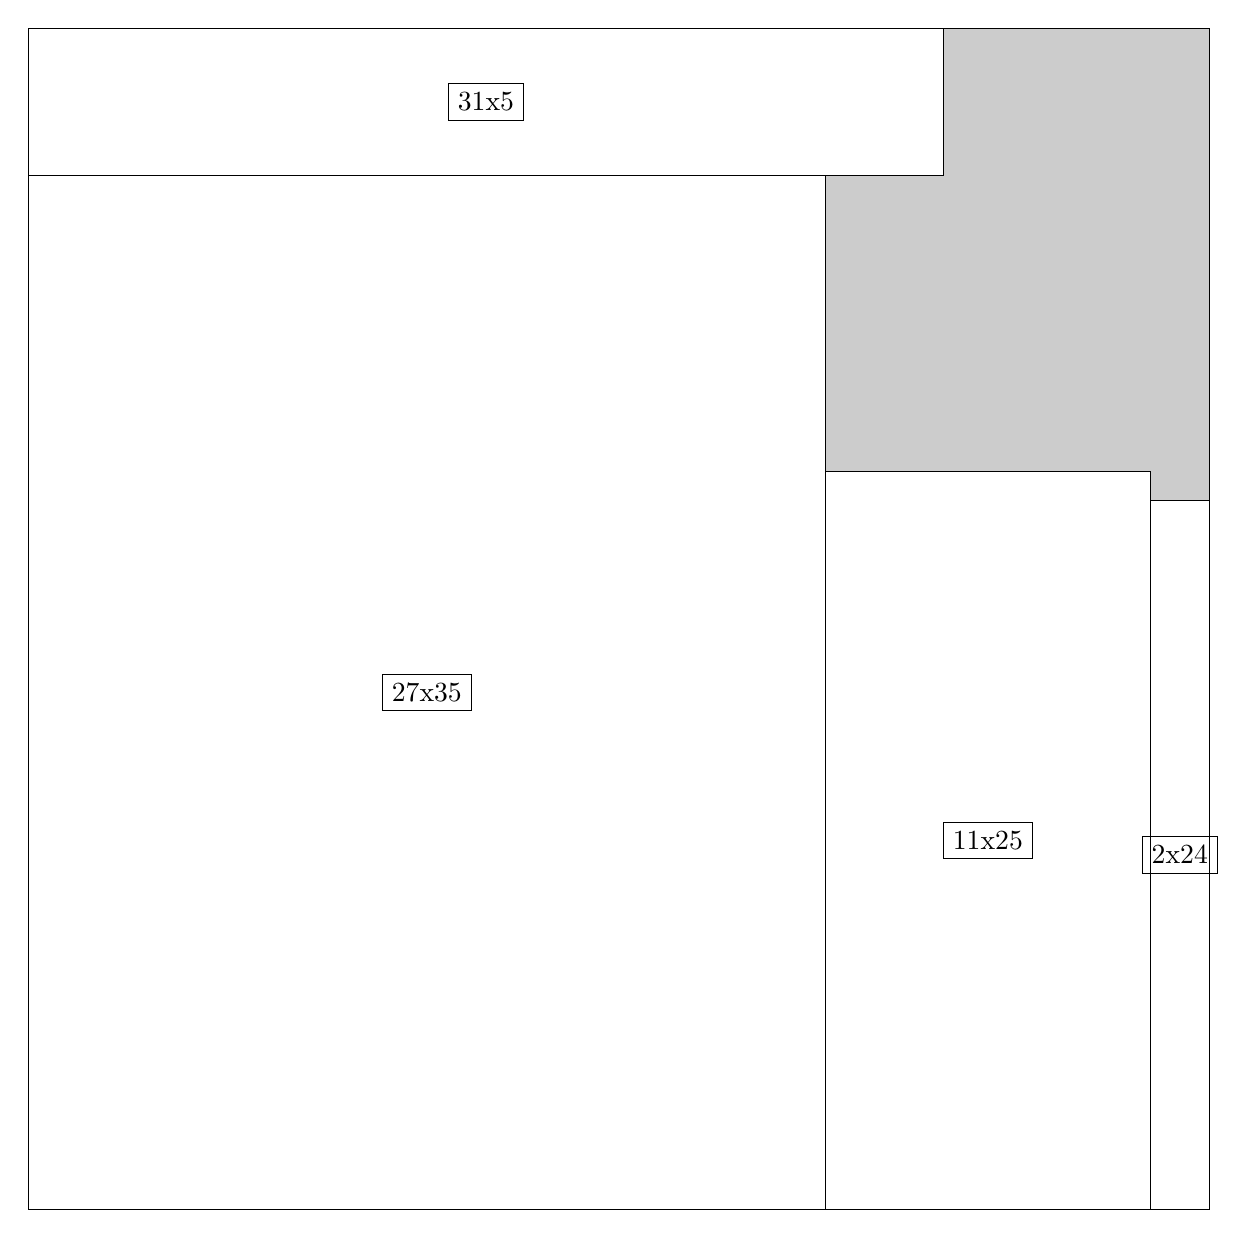
\begin{tikzpicture}[shorten >=1pt,scale=1.0,every node/.style={scale=1.0},->]
\tikzstyle{vertex}=[circle,fill=black!25,minimum size=14pt,inner sep=0pt]
\filldraw[fill=gray!40!white, draw=black] (0,0) rectangle (15.0,15.0);
\foreach \name/\x/\y/\w/\h in {27x35/0.0/0.0/10.125/13.125,11x25/10.125/0.0/4.125/9.375,31x5/0.0/13.125/11.625/1.875,2x24/14.25/0.0/0.75/9.0}
\filldraw[fill=white!40!white, draw=black] (\x,\y) rectangle node[draw] (\name) {\name} ++(\w,\h);
\end{tikzpicture}


w =27 , h =35 , x =0 , y =0 , v =945
\par
w =11 , h =25 , x =27 , y =0 , v =275
\par
w =31 , h =5 , x =0 , y =35 , v =155
\par
w =2 , h =24 , x =38 , y =0 , v =48
\par
\newpage


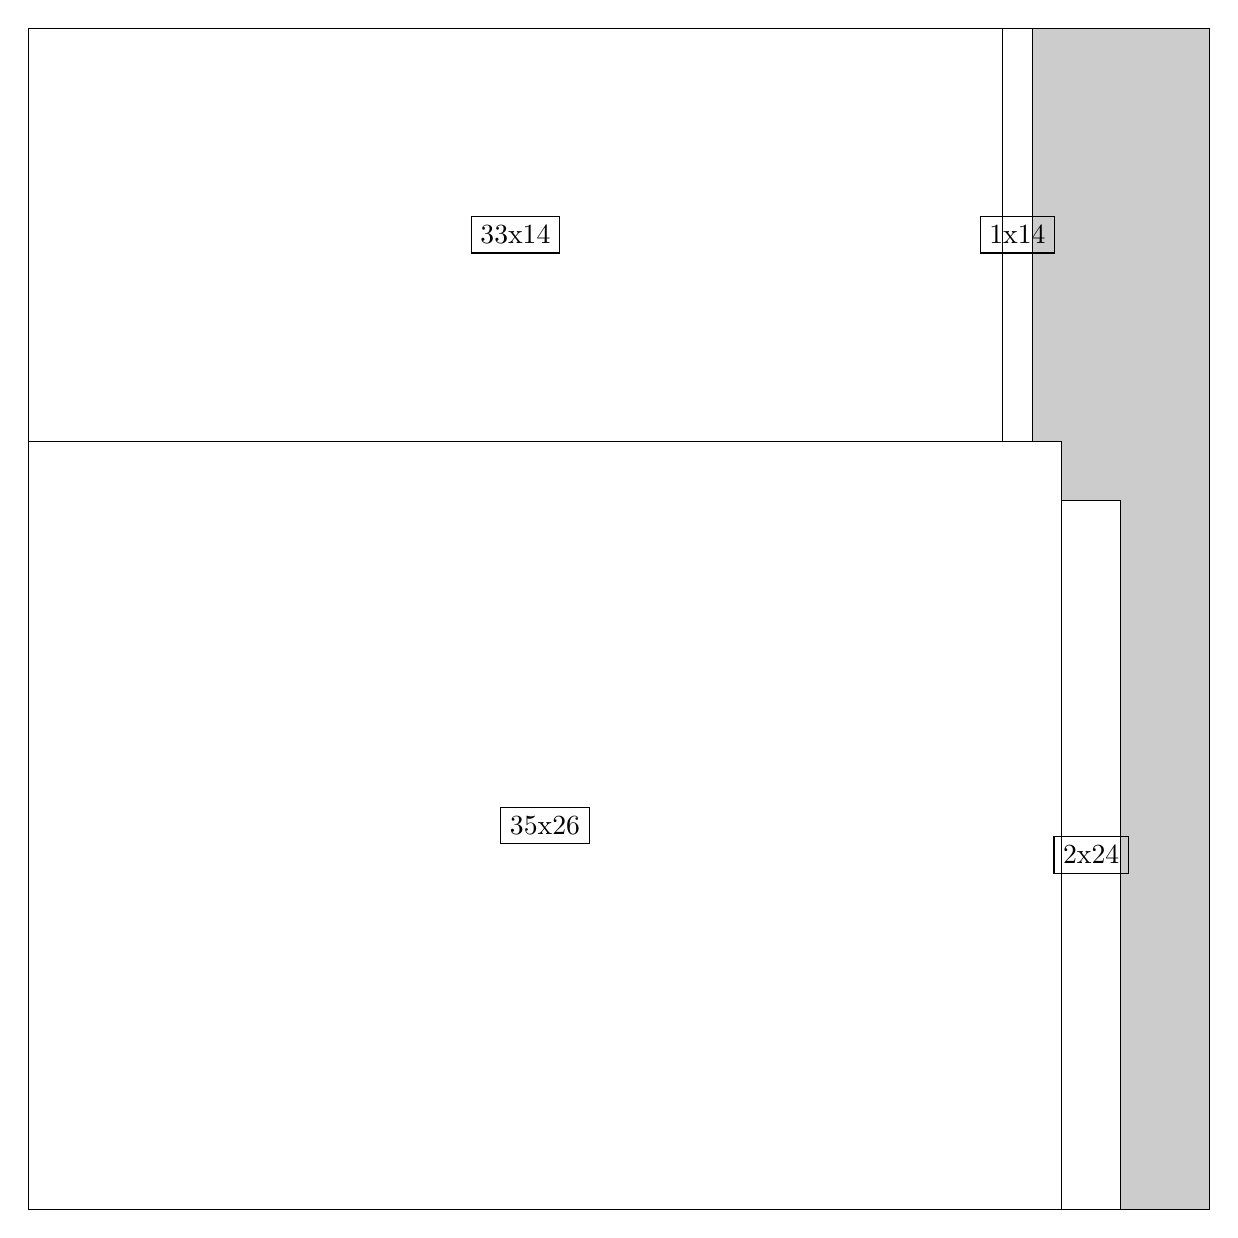
\begin{tikzpicture}[shorten >=1pt,scale=1.0,every node/.style={scale=1.0},->]
\tikzstyle{vertex}=[circle,fill=black!25,minimum size=14pt,inner sep=0pt]
\filldraw[fill=gray!40!white, draw=black] (0,0) rectangle (15.0,15.0);
\foreach \name/\x/\y/\w/\h in {35x26/0.0/0.0/13.125/9.75,33x14/0.0/9.75/12.375/5.25,2x24/13.125/0.0/0.75/9.0,1x14/12.375/9.75/0.375/5.25}
\filldraw[fill=white!40!white, draw=black] (\x,\y) rectangle node[draw] (\name) {\name} ++(\w,\h);
\end{tikzpicture}


w =35 , h =26 , x =0 , y =0 , v =910
\par
w =33 , h =14 , x =0 , y =26 , v =462
\par
w =2 , h =24 , x =35 , y =0 , v =48
\par
w =1 , h =14 , x =33 , y =26 , v =14
\par
\newpage


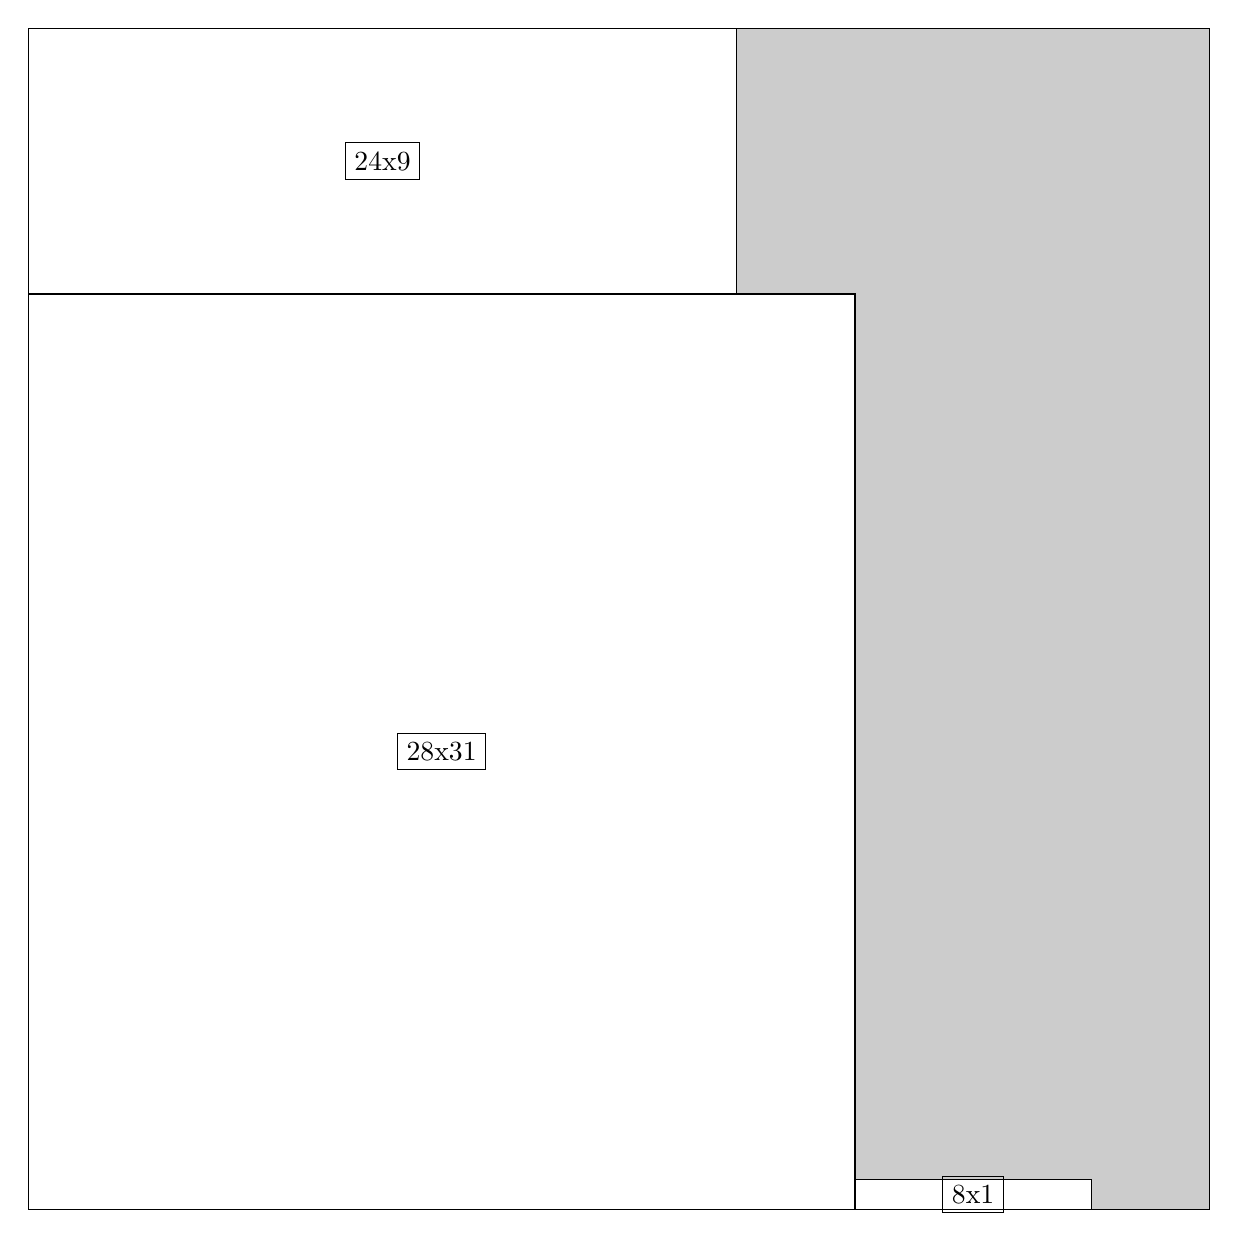
\begin{tikzpicture}[shorten >=1pt,scale=1.0,every node/.style={scale=1.0},->]
\tikzstyle{vertex}=[circle,fill=black!25,minimum size=14pt,inner sep=0pt]
\filldraw[fill=gray!40!white, draw=black] (0,0) rectangle (15.0,15.0);
\foreach \name/\x/\y/\w/\h in {28x31/0.0/0.0/10.5/11.625,24x9/0.0/11.625/9.0/3.375,8x1/10.5/0.0/3.0/0.375}
\filldraw[fill=white!40!white, draw=black] (\x,\y) rectangle node[draw] (\name) {\name} ++(\w,\h);
\end{tikzpicture}


w =28 , h =31 , x =0 , y =0 , v =868
\par
w =24 , h =9 , x =0 , y =31 , v =216
\par
w =8 , h =1 , x =28 , y =0 , v =8
\par
\newpage


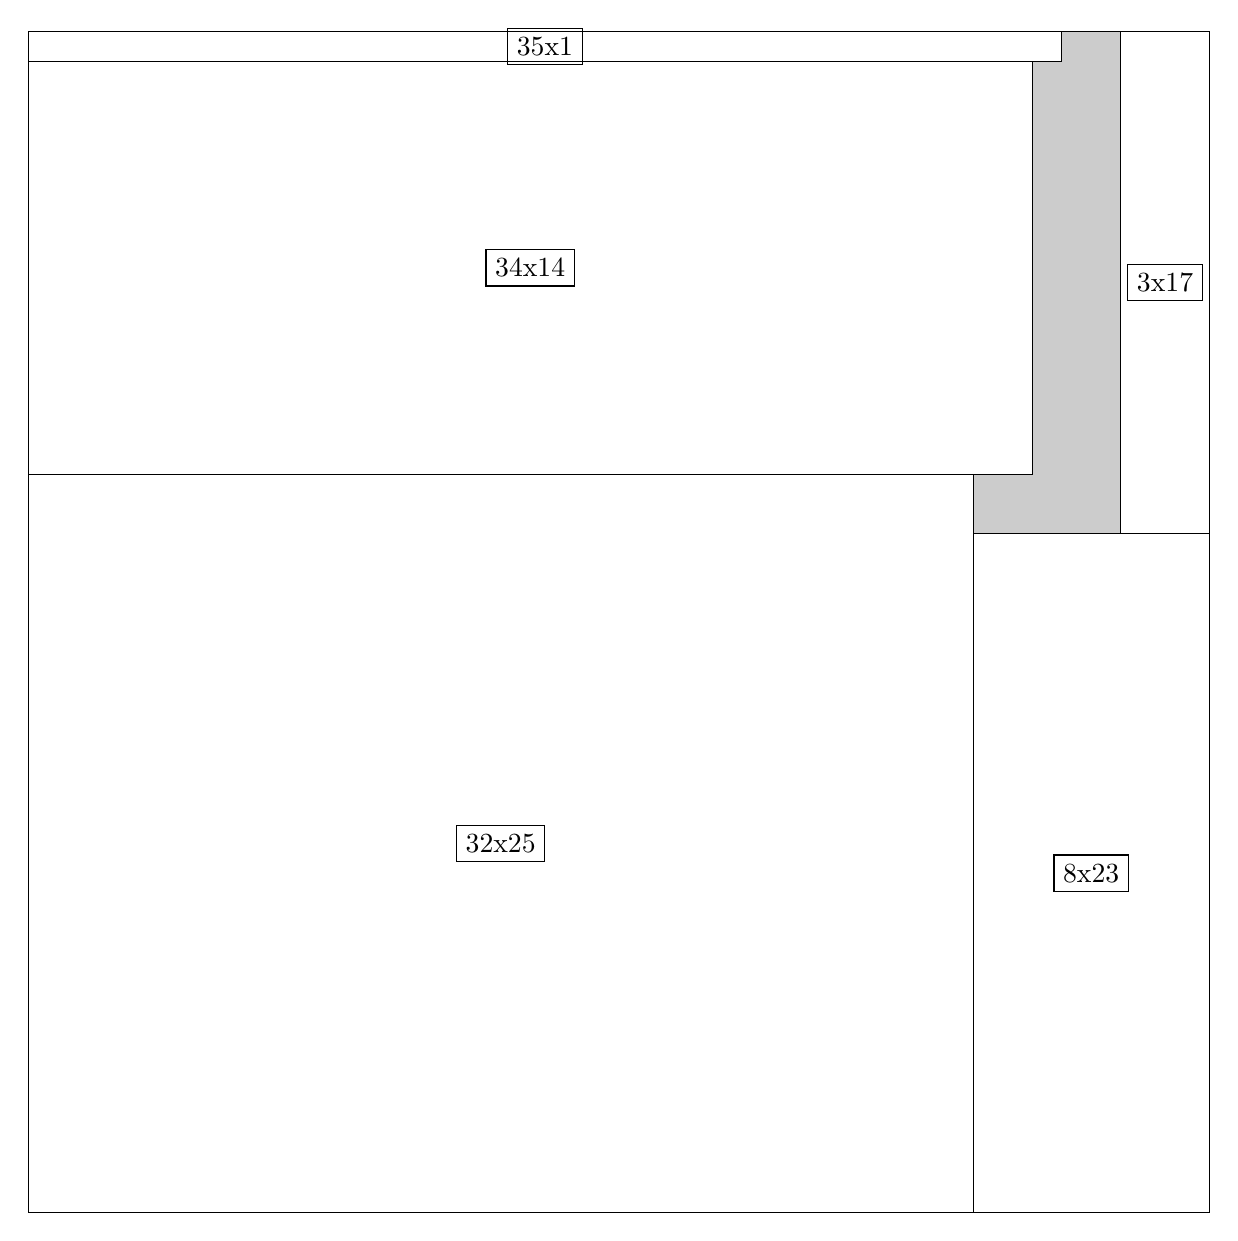
\begin{tikzpicture}[shorten >=1pt,scale=1.0,every node/.style={scale=1.0},->]
\tikzstyle{vertex}=[circle,fill=black!25,minimum size=14pt,inner sep=0pt]
\filldraw[fill=gray!40!white, draw=black] (0,0) rectangle (15.0,15.0);
\foreach \name/\x/\y/\w/\h in {32x25/0.0/0.0/12.0/9.375,8x23/12.0/0.0/3.0/8.625,34x14/0.0/9.375/12.75/5.25,3x17/13.875/8.625/1.125/6.375,35x1/0.0/14.625/13.125/0.375}
\filldraw[fill=white!40!white, draw=black] (\x,\y) rectangle node[draw] (\name) {\name} ++(\w,\h);
\end{tikzpicture}


w =32 , h =25 , x =0 , y =0 , v =800
\par
w =8 , h =23 , x =32 , y =0 , v =184
\par
w =34 , h =14 , x =0 , y =25 , v =476
\par
w =3 , h =17 , x =37 , y =23 , v =51
\par
w =35 , h =1 , x =0 , y =39 , v =35
\par
\newpage


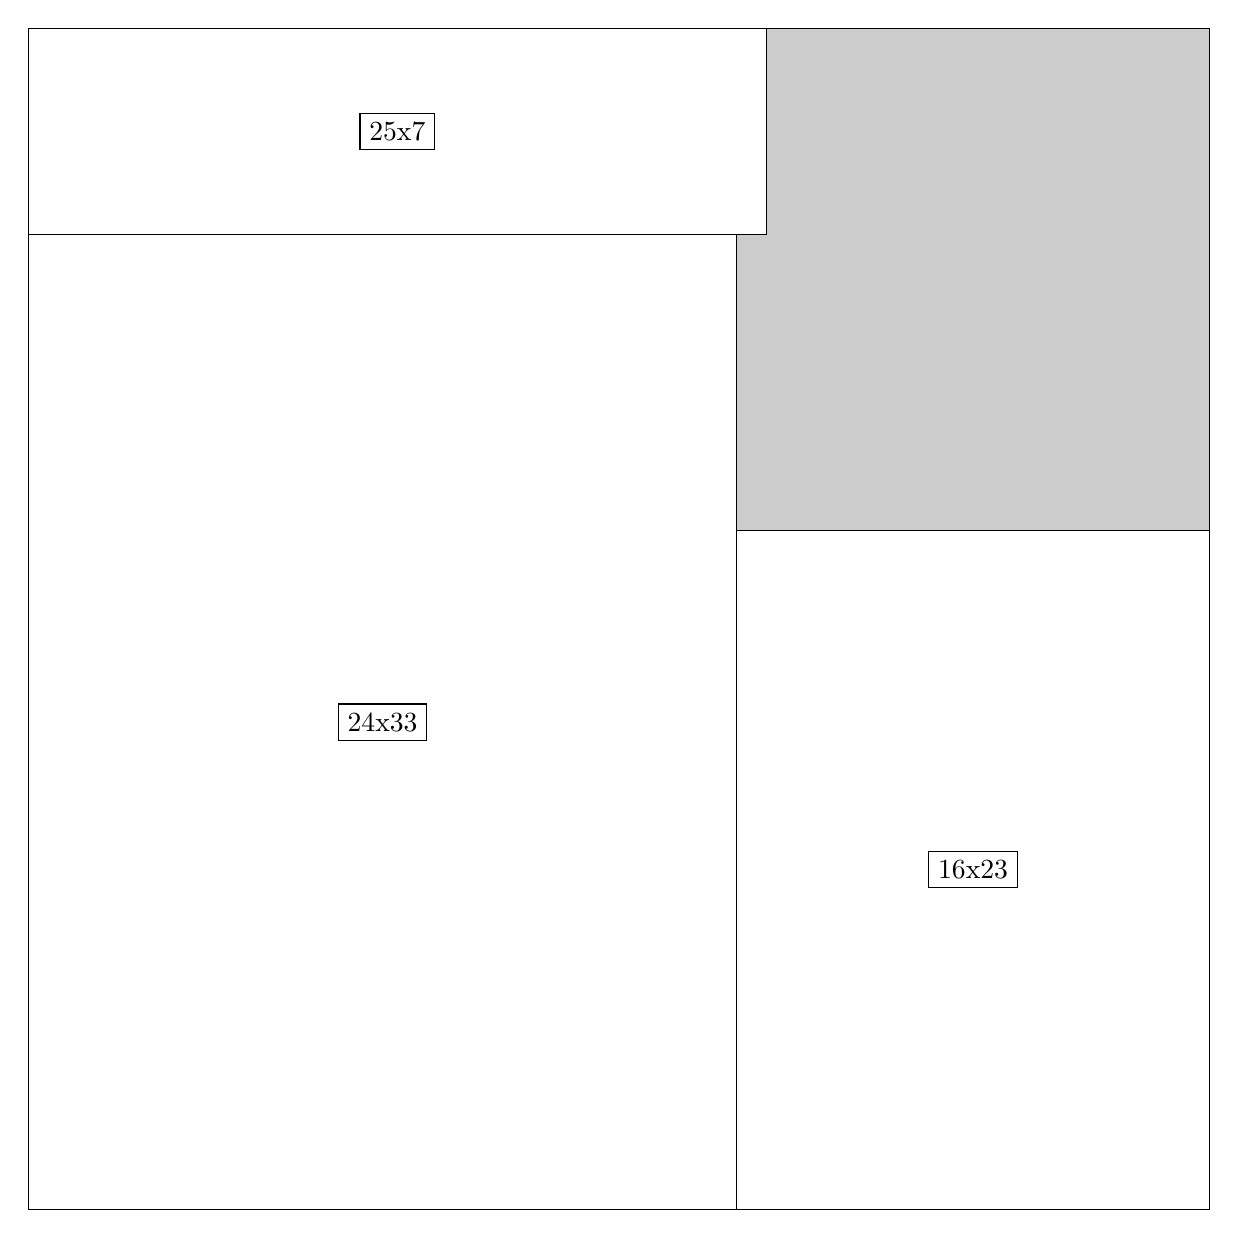
\begin{tikzpicture}[shorten >=1pt,scale=1.0,every node/.style={scale=1.0},->]
\tikzstyle{vertex}=[circle,fill=black!25,minimum size=14pt,inner sep=0pt]
\filldraw[fill=gray!40!white, draw=black] (0,0) rectangle (15.0,15.0);
\foreach \name/\x/\y/\w/\h in {24x33/0.0/0.0/9.0/12.375,16x23/9.0/0.0/6.0/8.625,25x7/0.0/12.375/9.375/2.625}
\filldraw[fill=white!40!white, draw=black] (\x,\y) rectangle node[draw] (\name) {\name} ++(\w,\h);
\end{tikzpicture}


w =24 , h =33 , x =0 , y =0 , v =792
\par
w =16 , h =23 , x =24 , y =0 , v =368
\par
w =25 , h =7 , x =0 , y =33 , v =175
\par
\newpage


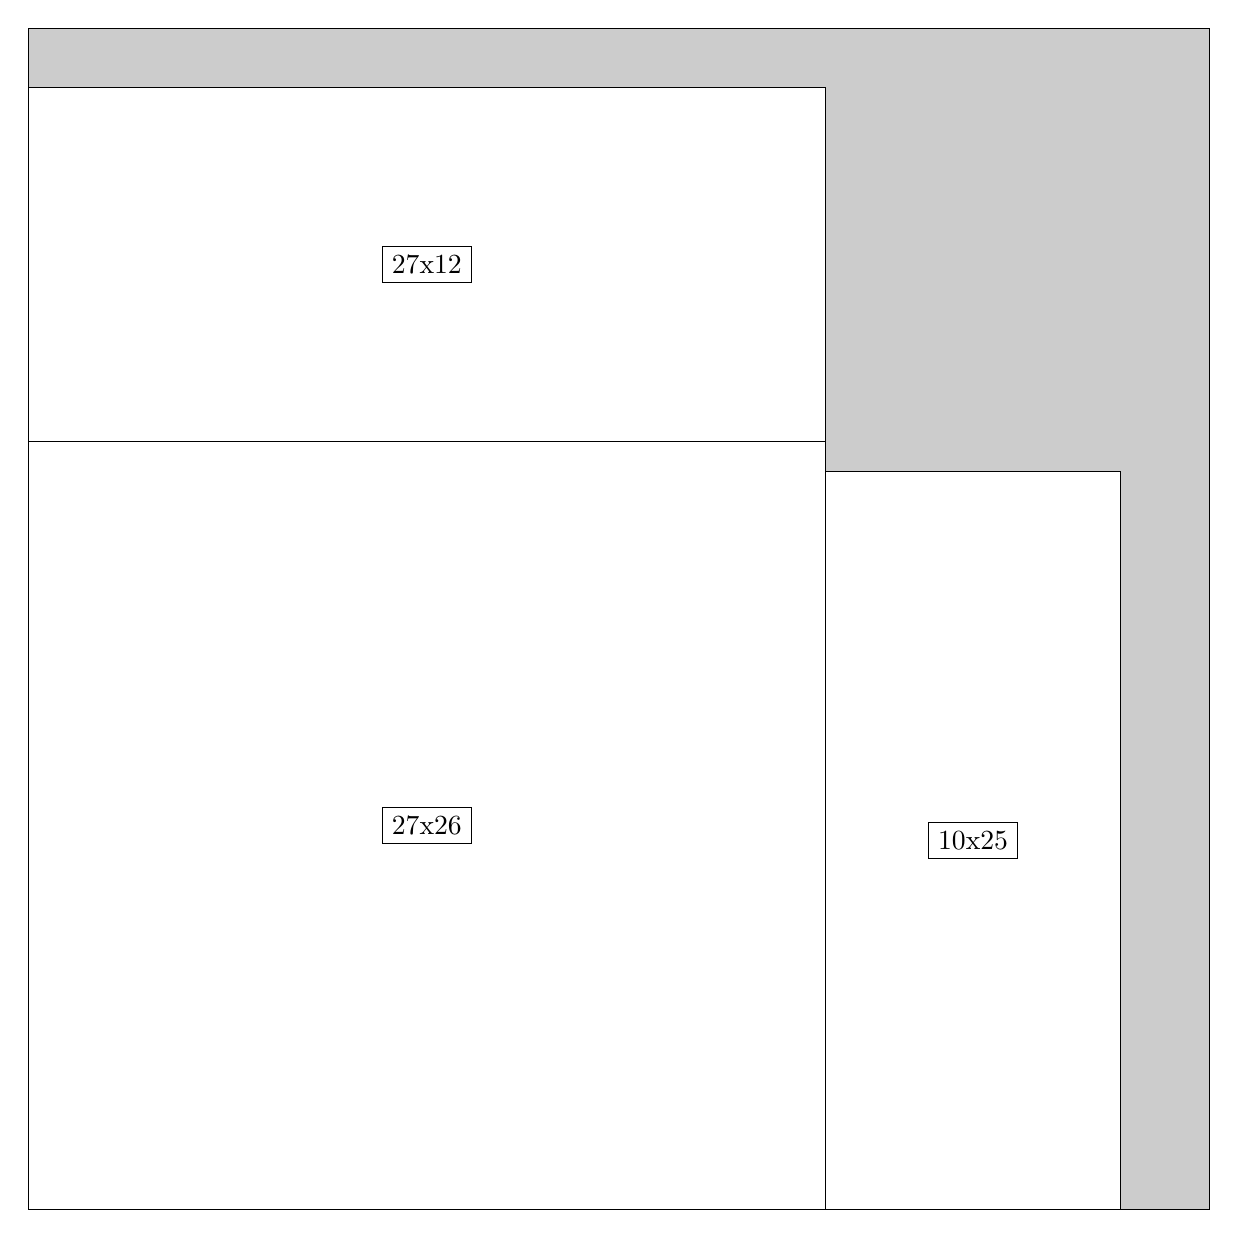
\begin{tikzpicture}[shorten >=1pt,scale=1.0,every node/.style={scale=1.0},->]
\tikzstyle{vertex}=[circle,fill=black!25,minimum size=14pt,inner sep=0pt]
\filldraw[fill=gray!40!white, draw=black] (0,0) rectangle (15.0,15.0);
\foreach \name/\x/\y/\w/\h in {27x26/0.0/0.0/10.125/9.75,27x12/0.0/9.75/10.125/4.5,10x25/10.125/0.0/3.75/9.375}
\filldraw[fill=white!40!white, draw=black] (\x,\y) rectangle node[draw] (\name) {\name} ++(\w,\h);
\end{tikzpicture}


w =27 , h =26 , x =0 , y =0 , v =702
\par
w =27 , h =12 , x =0 , y =26 , v =324
\par
w =10 , h =25 , x =27 , y =0 , v =250
\par
\newpage


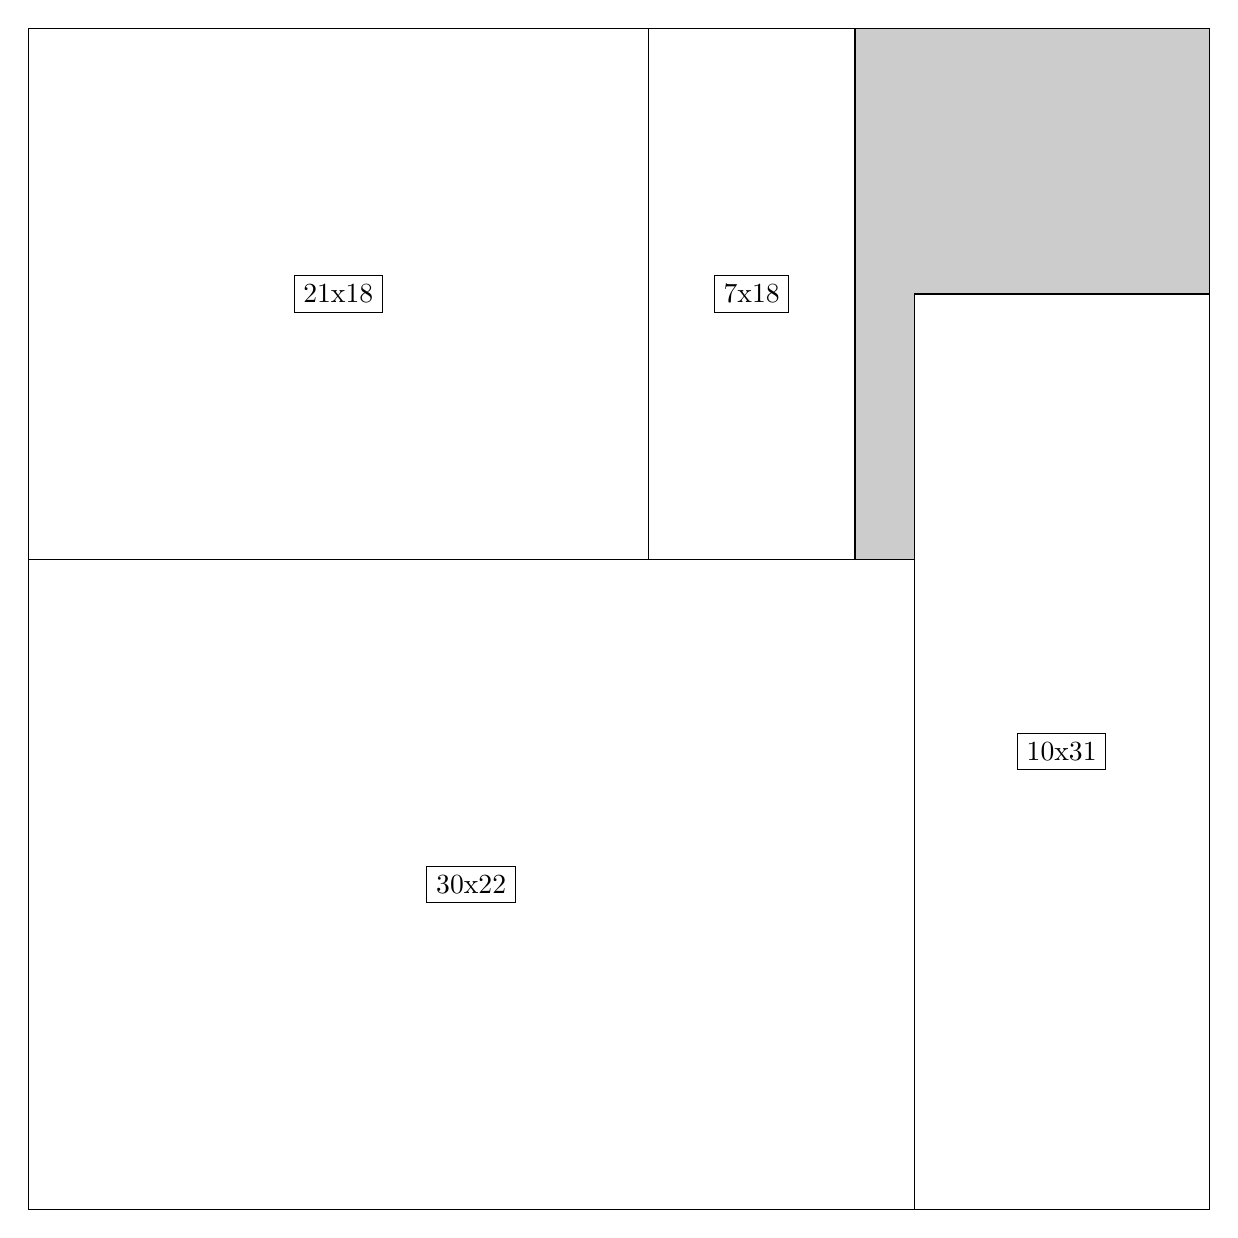
\begin{tikzpicture}[shorten >=1pt,scale=1.0,every node/.style={scale=1.0},->]
\tikzstyle{vertex}=[circle,fill=black!25,minimum size=14pt,inner sep=0pt]
\filldraw[fill=gray!40!white, draw=black] (0,0) rectangle (15.0,15.0);
\foreach \name/\x/\y/\w/\h in {30x22/0.0/0.0/11.25/8.25,21x18/0.0/8.25/7.875/6.75,10x31/11.25/0.0/3.75/11.625,7x18/7.875/8.25/2.625/6.75}
\filldraw[fill=white!40!white, draw=black] (\x,\y) rectangle node[draw] (\name) {\name} ++(\w,\h);
\end{tikzpicture}


w =30 , h =22 , x =0 , y =0 , v =660
\par
w =21 , h =18 , x =0 , y =22 , v =378
\par
w =10 , h =31 , x =30 , y =0 , v =310
\par
w =7 , h =18 , x =21 , y =22 , v =126
\par
\newpage


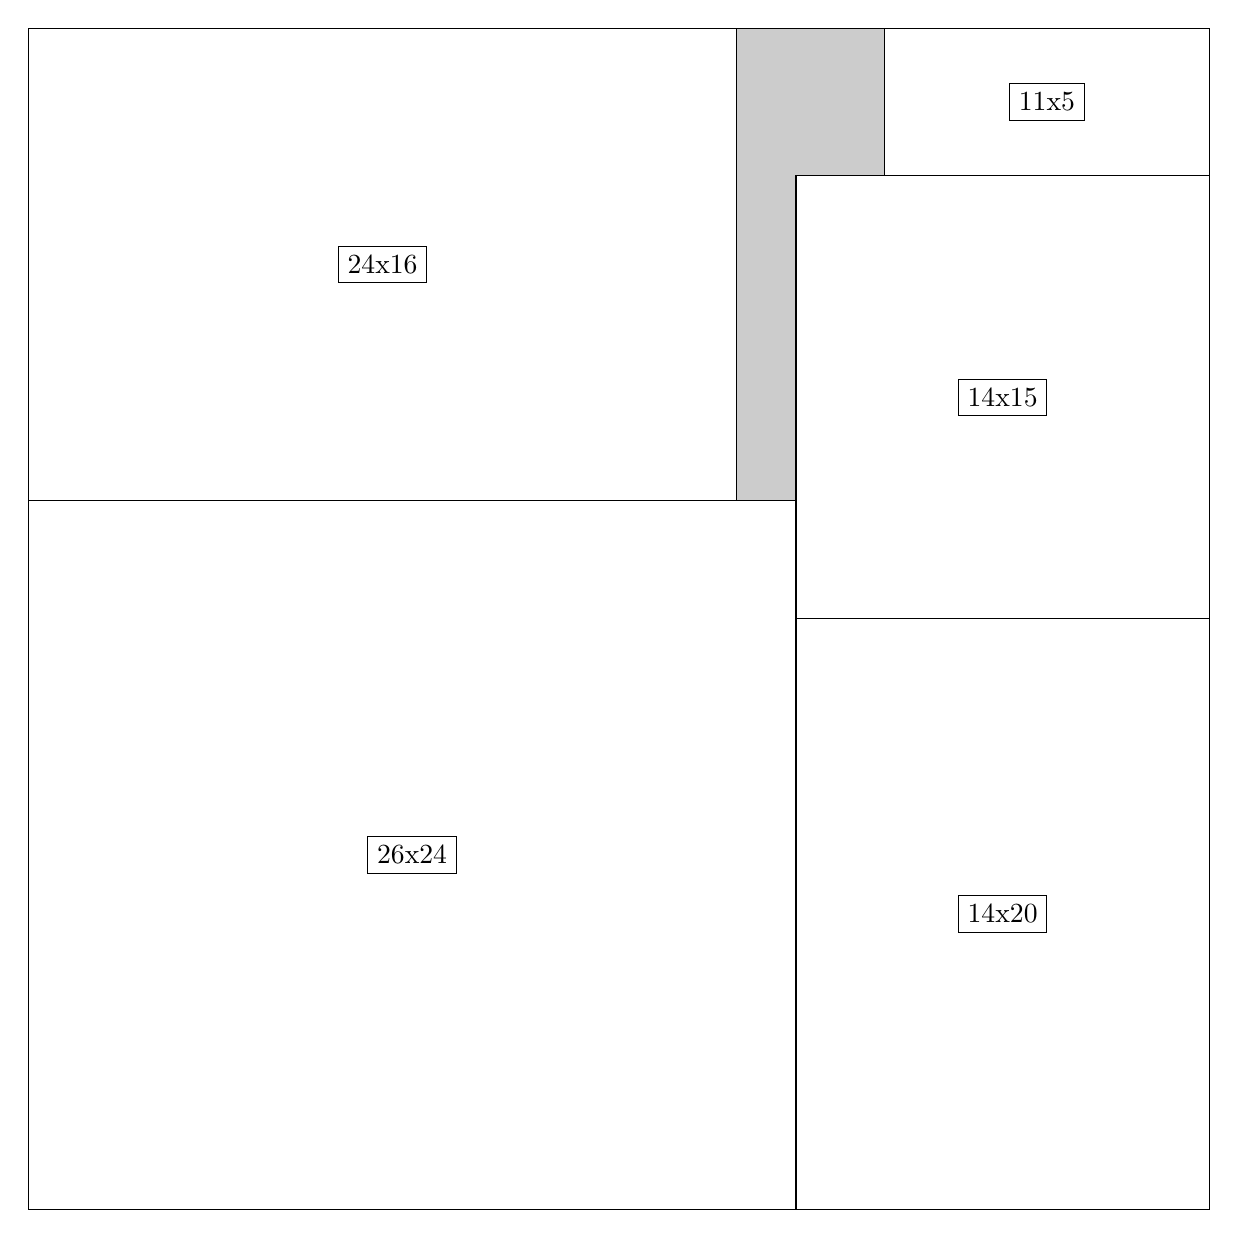
\begin{tikzpicture}[shorten >=1pt,scale=1.0,every node/.style={scale=1.0},->]
\tikzstyle{vertex}=[circle,fill=black!25,minimum size=14pt,inner sep=0pt]
\filldraw[fill=gray!40!white, draw=black] (0,0) rectangle (15.0,15.0);
\foreach \name/\x/\y/\w/\h in {26x24/0.0/0.0/9.75/9.0,11x5/10.875/13.125/4.125/1.875,24x16/0.0/9.0/9.0/6.0,14x20/9.75/0.0/5.25/7.5,14x15/9.75/7.5/5.25/5.625}
\filldraw[fill=white!40!white, draw=black] (\x,\y) rectangle node[draw] (\name) {\name} ++(\w,\h);
\end{tikzpicture}


w =26 , h =24 , x =0 , y =0 , v =624
\par
w =11 , h =5 , x =29 , y =35 , v =55
\par
w =24 , h =16 , x =0 , y =24 , v =384
\par
w =14 , h =20 , x =26 , y =0 , v =280
\par
w =14 , h =15 , x =26 , y =20 , v =210
\par
\newpage


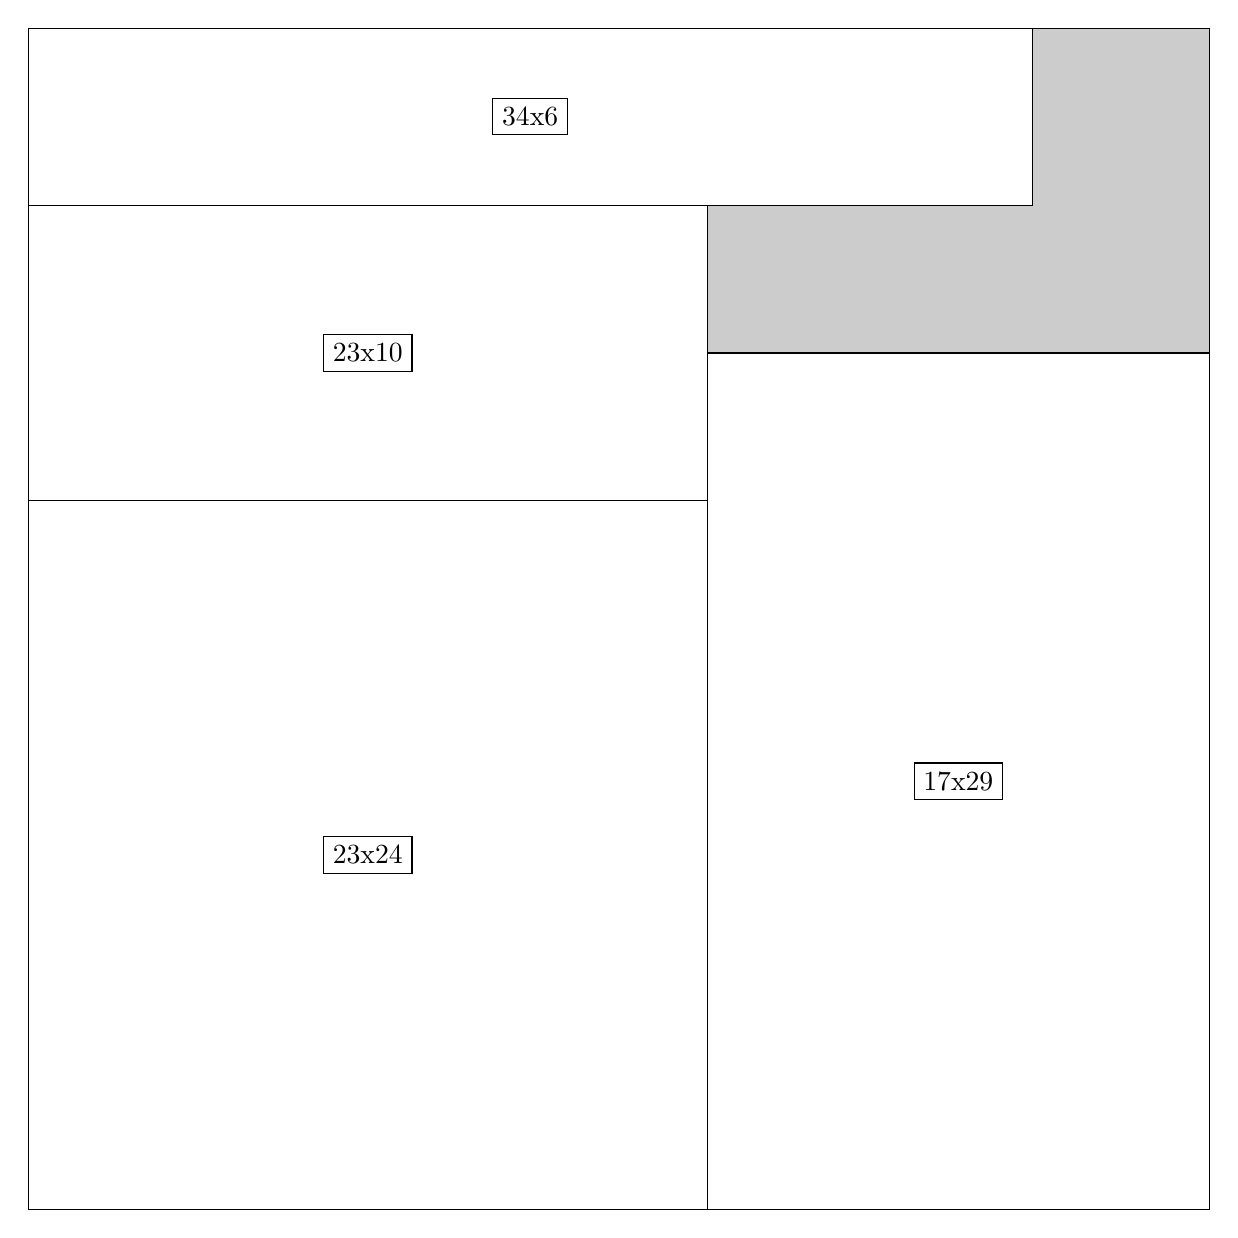
\begin{tikzpicture}[shorten >=1pt,scale=1.0,every node/.style={scale=1.0},->]
\tikzstyle{vertex}=[circle,fill=black!25,minimum size=14pt,inner sep=0pt]
\filldraw[fill=gray!40!white, draw=black] (0,0) rectangle (15.0,15.0);
\foreach \name/\x/\y/\w/\h in {23x24/0.0/0.0/8.625/9.0,17x29/8.625/0.0/6.375/10.875,23x10/0.0/9.0/8.625/3.75,34x6/0.0/12.75/12.75/2.25}
\filldraw[fill=white!40!white, draw=black] (\x,\y) rectangle node[draw] (\name) {\name} ++(\w,\h);
\end{tikzpicture}


w =23 , h =24 , x =0 , y =0 , v =552
\par
w =17 , h =29 , x =23 , y =0 , v =493
\par
w =23 , h =10 , x =0 , y =24 , v =230
\par
w =34 , h =6 , x =0 , y =34 , v =204
\par
\newpage


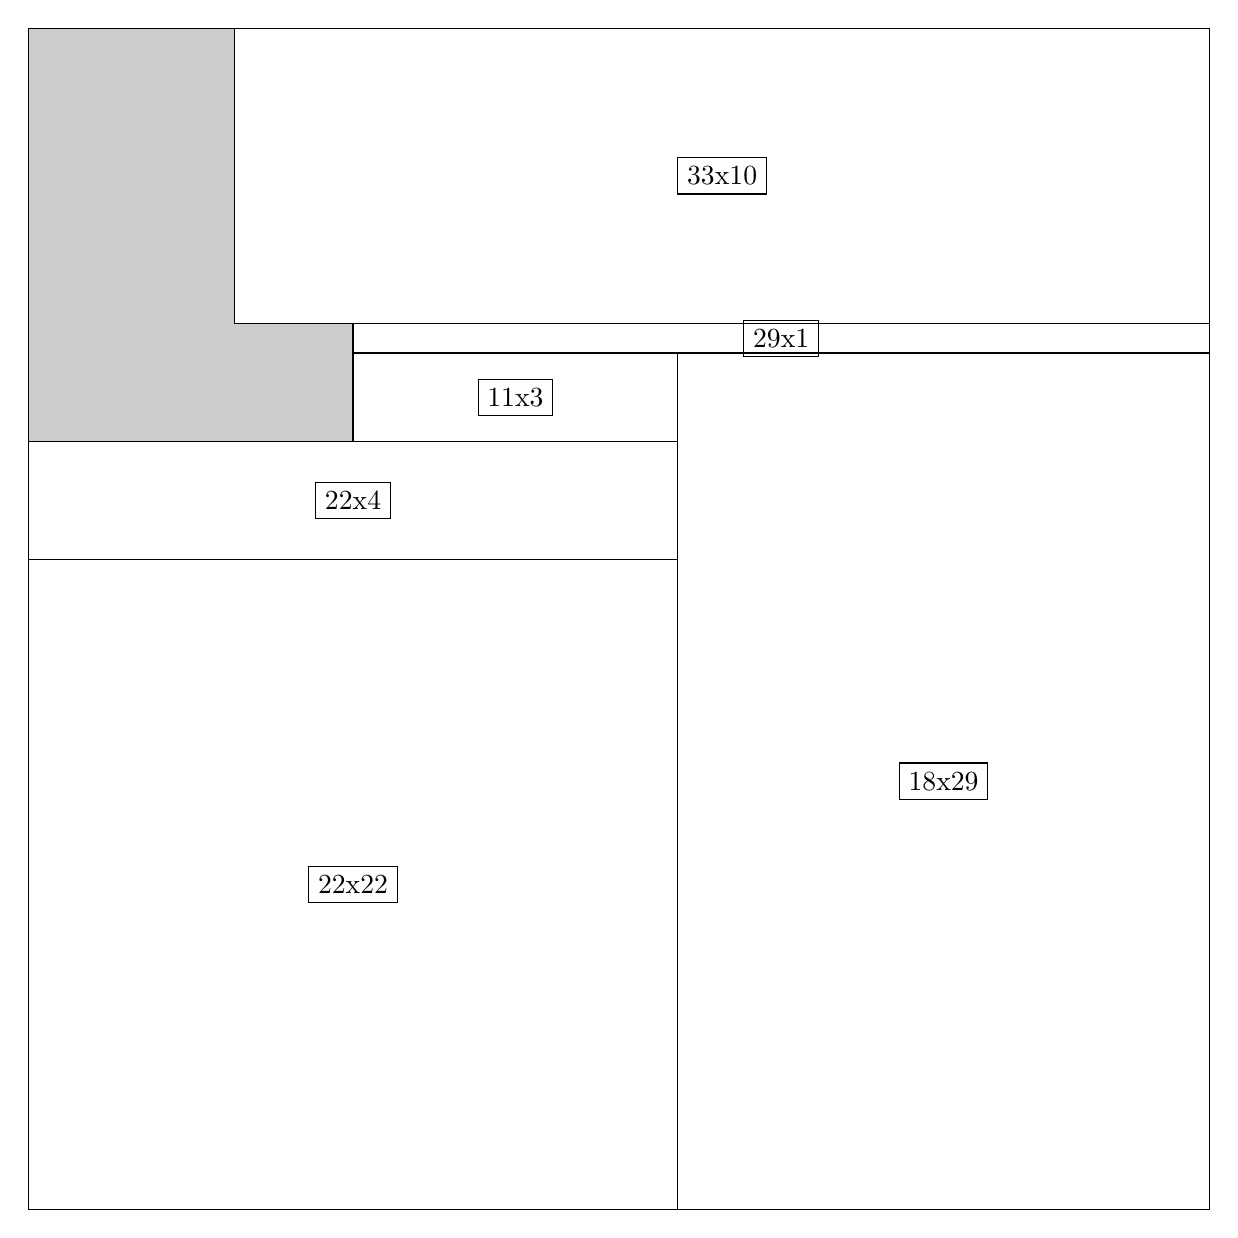
\begin{tikzpicture}[shorten >=1pt,scale=1.0,every node/.style={scale=1.0},->]
\tikzstyle{vertex}=[circle,fill=black!25,minimum size=14pt,inner sep=0pt]
\filldraw[fill=gray!40!white, draw=black] (0,0) rectangle (15.0,15.0);
\foreach \name/\x/\y/\w/\h in {18x29/8.25/0.0/6.75/10.875,22x22/0.0/0.0/8.25/8.25,33x10/2.625/11.25/12.375/3.75,22x4/0.0/8.25/8.25/1.5,11x3/4.125/9.75/4.125/1.125,29x1/4.125/10.875/10.875/0.375}
\filldraw[fill=white!40!white, draw=black] (\x,\y) rectangle node[draw] (\name) {\name} ++(\w,\h);
\end{tikzpicture}


w =18 , h =29 , x =22 , y =0 , v =522
\par
w =22 , h =22 , x =0 , y =0 , v =484
\par
w =33 , h =10 , x =7 , y =30 , v =330
\par
w =22 , h =4 , x =0 , y =22 , v =88
\par
w =11 , h =3 , x =11 , y =26 , v =33
\par
w =29 , h =1 , x =11 , y =29 , v =29
\par
\newpage


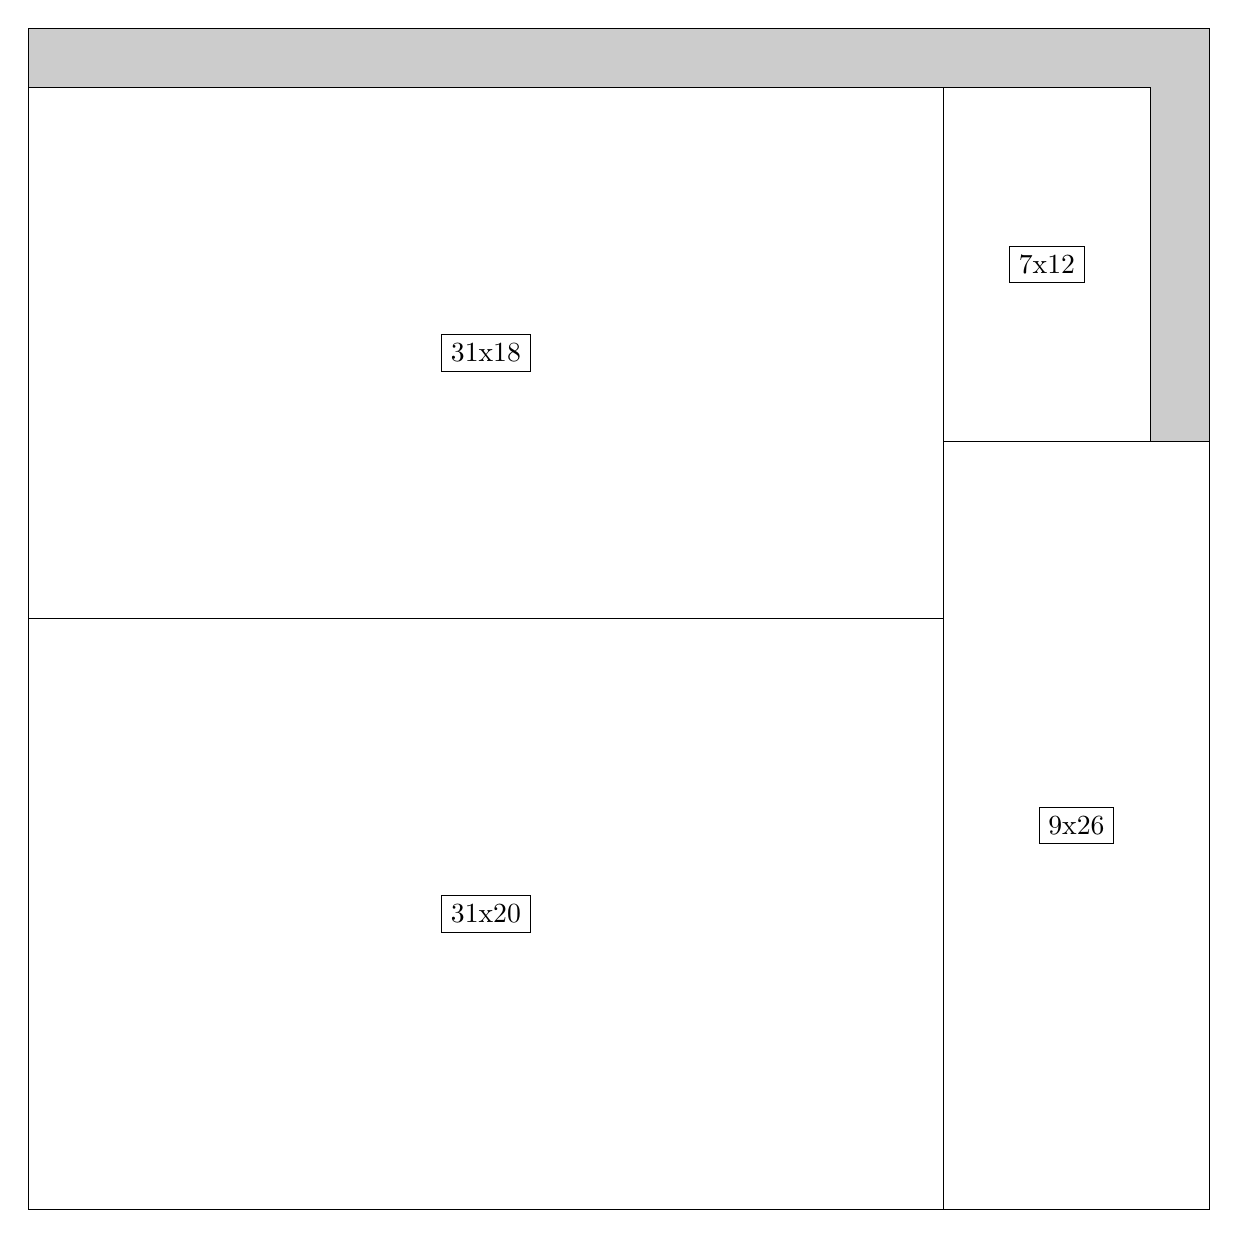
\begin{tikzpicture}[shorten >=1pt,scale=1.0,every node/.style={scale=1.0},->]
\tikzstyle{vertex}=[circle,fill=black!25,minimum size=14pt,inner sep=0pt]
\filldraw[fill=gray!40!white, draw=black] (0,0) rectangle (15.0,15.0);
\foreach \name/\x/\y/\w/\h in {31x20/0.0/0.0/11.625/7.5,31x18/0.0/7.5/11.625/6.75,9x26/11.625/0.0/3.375/9.75,7x12/11.625/9.75/2.625/4.5}
\filldraw[fill=white!40!white, draw=black] (\x,\y) rectangle node[draw] (\name) {\name} ++(\w,\h);
\end{tikzpicture}


w =31 , h =20 , x =0 , y =0 , v =620
\par
w =31 , h =18 , x =0 , y =20 , v =558
\par
w =9 , h =26 , x =31 , y =0 , v =234
\par
w =7 , h =12 , x =31 , y =26 , v =84
\par
\newpage


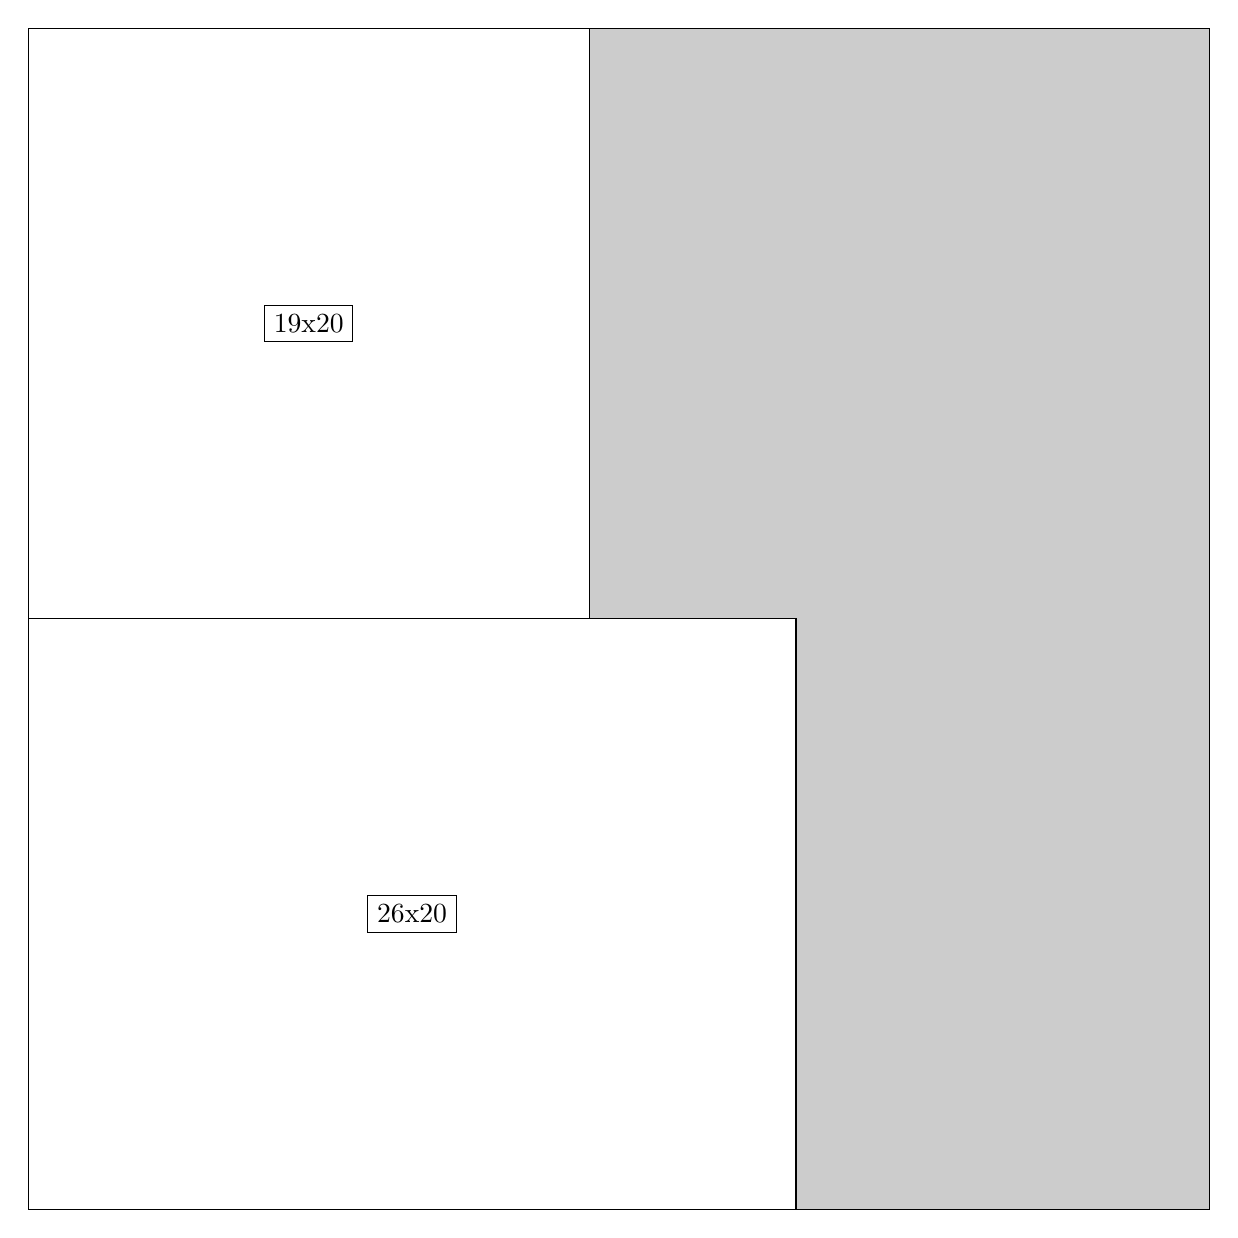
\begin{tikzpicture}[shorten >=1pt,scale=1.0,every node/.style={scale=1.0},->]
\tikzstyle{vertex}=[circle,fill=black!25,minimum size=14pt,inner sep=0pt]
\filldraw[fill=gray!40!white, draw=black] (0,0) rectangle (15.0,15.0);
\foreach \name/\x/\y/\w/\h in {26x20/0.0/0.0/9.75/7.5,19x20/0.0/7.5/7.125/7.5}
\filldraw[fill=white!40!white, draw=black] (\x,\y) rectangle node[draw] (\name) {\name} ++(\w,\h);
\end{tikzpicture}


w =26 , h =20 , x =0 , y =0 , v =520
\par
w =19 , h =20 , x =0 , y =20 , v =380
\par
\newpage


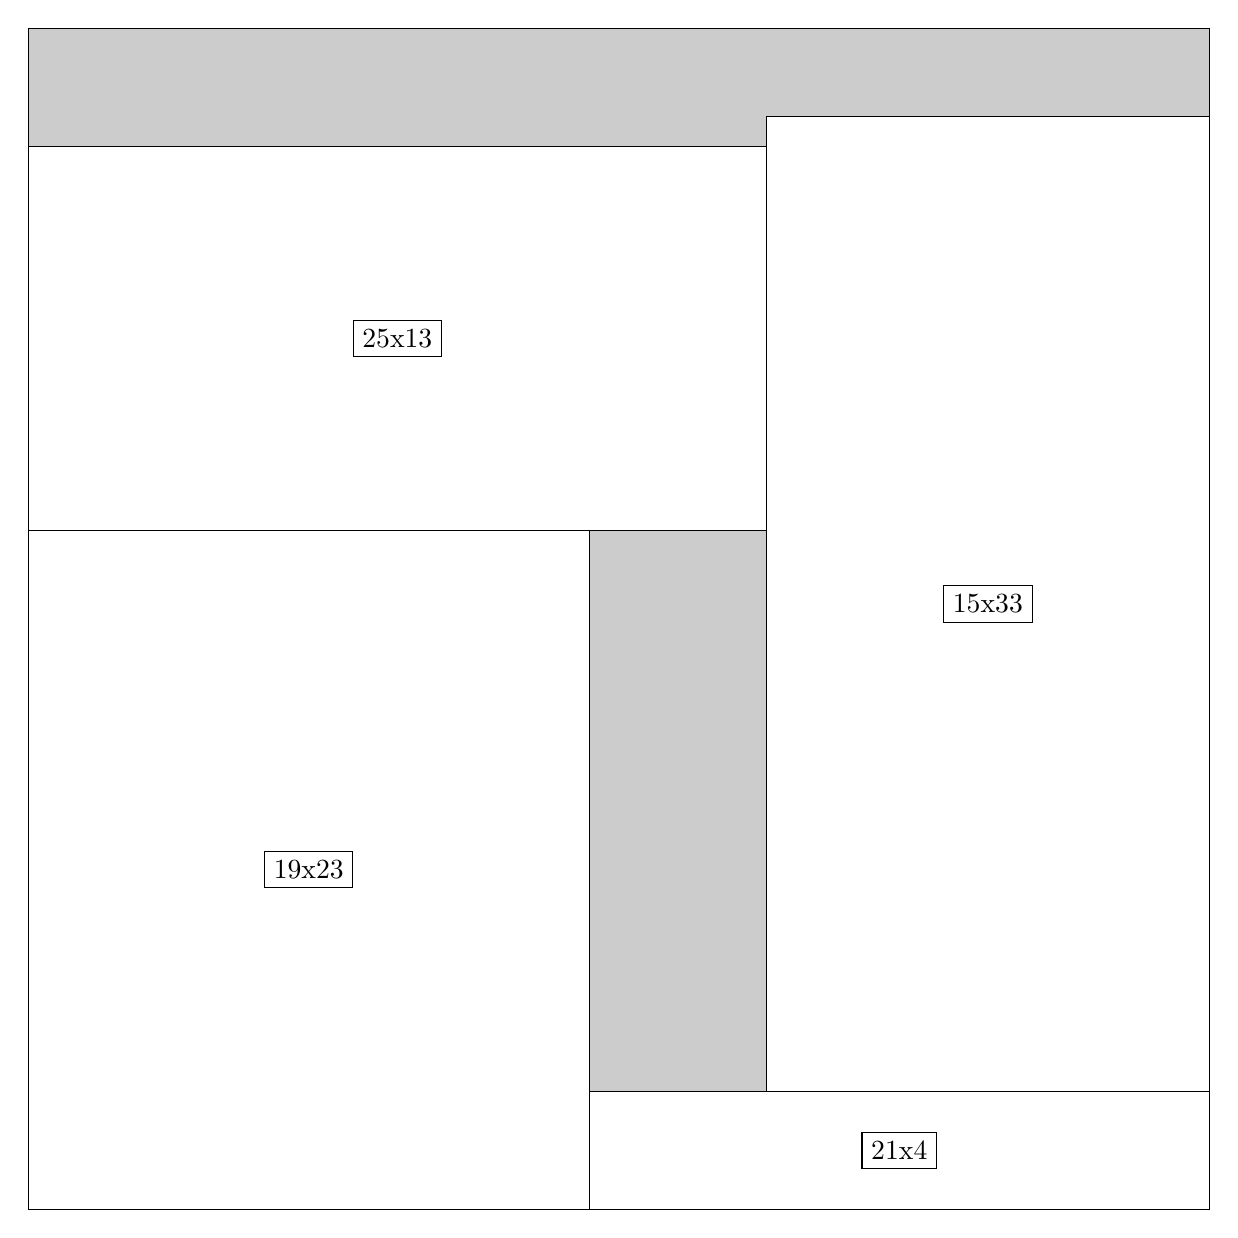
\begin{tikzpicture}[shorten >=1pt,scale=1.0,every node/.style={scale=1.0},->]
\tikzstyle{vertex}=[circle,fill=black!25,minimum size=14pt,inner sep=0pt]
\filldraw[fill=gray!40!white, draw=black] (0,0) rectangle (15.0,15.0);
\foreach \name/\x/\y/\w/\h in {19x23/0.0/0.0/7.125/8.625,15x33/9.375/1.5/5.625/12.375,25x13/0.0/8.625/9.375/4.875,21x4/7.125/0.0/7.875/1.5}
\filldraw[fill=white!40!white, draw=black] (\x,\y) rectangle node[draw] (\name) {\name} ++(\w,\h);
\end{tikzpicture}


w =19 , h =23 , x =0 , y =0 , v =437
\par
w =15 , h =33 , x =25 , y =4 , v =495
\par
w =25 , h =13 , x =0 , y =23 , v =325
\par
w =21 , h =4 , x =19 , y =0 , v =84
\par
\newpage


\end{document}